\chapter{Senzory}
Ke dni odevzdání práce je funkční všesměrový ultrazvukový senzor, a~to ve dvou iteracích.
Dále je funkční také sběrač ultrazvukových senzorů.
Další senzory jsou ve vývoji.

\section{Všesměrový ultrazvukový senzor}
Obě iterace tohoto senzoru používají 8 senzorů HC-SR04 uspořádaných do osmiúhelníku.
Hlavní rozdíl mezi nimi je v~možnosnosti použití.
Zatímco první iterace je nachystaná pro singleplayerové disciplíny,~druhá iterace, pracovně pojmenovaná Janus omni-ultra vyžaduje buď soupeře na hřišti, nebo možnost umístění majáčků okolo hřiště. 
Na Pražském robotickém dni tomuto odpovídá pouze disciplína Roadside Assistance Advanced\cite{roadside}, ve světě jsou však tyto disciplíny rozšířenější.

\subsection{Singleplayerové řešení}
Jedná se o~osm senzorů HC-SR04 uspořádaných do osmiúhelníku, všechny senzory jsou svedeny do procesoru tak, aby se každý dal číst a~aktivovat samostatně.
Senzor musí být na robotovi uchycen nad úrovní všech ostatních jednotek, potřebuje mít 360$^{\circ}$ výhled.
Druhý požadavek na použití tohoto senzoru je výškový rozdíl měřených objektů a~objektů, které se na hřišti nacházejí, ale vzdálenost od nich k~robotovi měřit nechceme.
Senzor musí být umístěn tak, aby jeho vrchní plocha byla maximálně na úrovni vrchní plochy měřených objektů, ale zároveň tak, aby při měření nezabíraly nechtěné objekty, což už je ovšem potřeba vyzkoušet na každém hřišti samostatně.

Oproti samostatně používaným senzorům má toto řešení zásadní výhodu hlavně co se náročnosti na čas procesoru týká.
Při přímém připojení na řídící jednotku musí jednotka při každém průchodu vyčíst všech 8 senzorů, kdy každé měření jednoho senzoru může trvat na běžném hřišti až 16~ms, tento čas se může zdát zanedbatelný, ale při provozu robota tomu tak není.
Použijeme-li dodatečný meziprocesor, tento čas nezměníme, ale hlavní jednotka se již samotným měřením nemusí zabývat, pouze pošle požadavek na modul a~ten jí, podle předem nastavešných kritérií, vrátí buď všechny hodnoty, které jsou již v~modulu změřené a~nachystané, nebo pouze tu nejmenší.
Nabízí se také možnost nechat se pouze upozornit v~případě, že některá ze vzdáleností na naměřených modulem překročí předem danou mez.
Tímto způsobem se celý proces, jak měření jako takového, tak programování robota, razantně zjednodušuje.  

\subsection{Janus omni-ultra}
Tento senzor, nebo lépe řečeno uspořádání, potřebuje ke svému fungování dvě stanice.
Jedna ze stanic je umístěna na robotovi, nazveme ji přijímačem.
Druhá stanice je umístěna na soupeři, případně na pozici pro majáček na okraji hřiště, nazveme ji vysílačem.
Obě stanice jsou založeny na singleplayerovém řešení.

\subsubsection{Vysílač}
Vysílač sestává ze singleplayerové verze, kruhu synchronizačních IR LED, baterie a~řídící desky.
Jako baterie je zde použit dvoučlánek baterií 18650.
Řídící deska sestává ze dvou DPS umístěných nad sebou, propojených šestipinovým konektorem.

Na horní desce se nachází procesor a~náležitosti potřebné k~jeho fungování.
Jako procesor je zde zvolen ATMEGA328 \cite{atmega}, není zde totiž potřeba komunikace po Janus protocol, není tedu nutné používat dražší ESP32.
Pro toto použití je ATMEGA dostačující.
Úkolem procesoru je poslat na 40~kHz modulovaný puls ze synchronizačních IR LED společně s~vysláním ultrazvukového signálu ze všech HC-SR04 naráz. 
Není třeba měřit návratový čas, protože na vysílači nás nezajímá.
Procesor má zároveň dvě signalizační LED a~umožňuje měření baterií, v~případě vybití signalizuje tuto skutečnost.

Na spodní desce se nachází kruh synchronizačních IR LED, spojených na jeden tranzistor.
Dále se zde nachází stabilizátor AMS1117 5V \cite{ams1117}, ten upravuje napětí z~baterií pro potřeby procesoru.

\begin{figure}
    \begin{small}
        \begin{center}
            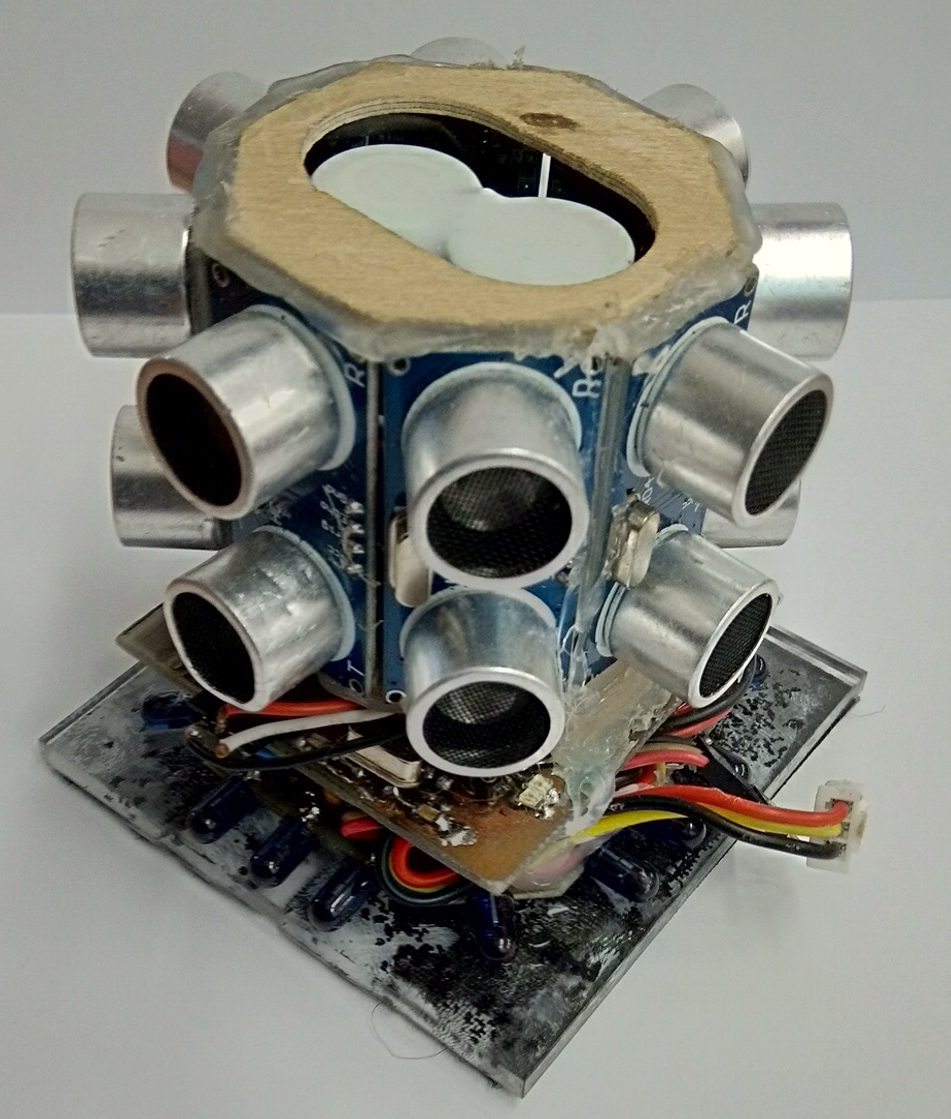
\includegraphics[width=250px, angle = 0, scale = 0.7]{img/Vysilac2.jpg}
        \end{center}
        \caption{Vysílač}
        \label{fig: Ultrasonic}
    \end{small}
\end{figure}


\subsubsection{Přijímač}
Přijímač sestává ze singleplayerové verze, kruhu osmi IR přijímačů TSOP4840 a~řídící jednotky.
Všechny HC-SR04 mají znefunkčněný vysílač.
Když procesor přijme z~IR přijímačů signál, započne měřit čas a~odešle vysílací puls do HC-SR04, poté již jen čeká než se změní hodnota některého z~Echo pinů na HC-SR04.
V~okamžiku, kdy se tak stane, procesor ukončí měření času a~zaznamená si, ze kterého HC-SR04 změna přišla.
Díky tomu je schopen senzor zjistit nejen vzdálenost od vysílače, ale i přibližný směr k~němu.
Cokoliv, co přijde po první změně nás nezajímá, protože se jedná o~náhodný odraz od objektů v~prostředí.

\section{Sběrač ultrazvukových senzorů}\label{Sberac}
Tento senzor používá řídící elektroniku singleplayerového řešení všesměrového senzoru.
Hlavní rozdíl oproti němu je možnost libovolného umístění senzorů HC-SR04 na robota.
Důvodem tvorby tohoto senzoru je časová náročnost měření jednotlivých senzorů, která může razantně ovlivnit reakční dobu robota.
Senzor je navíc oproti singlplayerovému řešení schopen po softwarovém zapnutí této funkce odesílat interupt signál při překročení nastavené meze přiblížení pro některý z~HC-SR04.